% !TEX root = ../../../main.tex
% 来源：中学数学实验教材·第三册（高中数学）
% 章节：任意角的三角函数 / 三角函数的诱导公式
% 原始文件：6.tex，行 2096-2114
% 类型：tikz
% ---
\begin{tikzpicture}[>=latex, scale=1.3]
    \draw[->](-2,0)--(2.5,0)node[right]{$x$};
    \draw[->](0,-2)--(0,2)node[right]{$y$};
    \draw (0,0) circle(1.5);
    \draw[very thick] (150:1.5)node[left]{$P_1$}--(-30:1.5)node[left]{$P_2$}--(1.5,-1.732/2);

\draw [<->|](1.6, 0)--node[right]{$\tfrac{\sqrt{3}}{3}$}(1.6,-1.732/2);
\draw [<->|](1.6, 0)--node[right]{$\tfrac{\sqrt{3}}{3}$}(1.6,1.732/2);



\node at (1.5,-1.732/2-.3)[right]{$L\left(1,-\tfrac{\sqrt{3}}{3}\right)$};

    \node at (-.25,-.25){$O$};
    \draw[dashed] (0,0)--(30:1.5)--(1.5,1.732/2);
\draw (1.5,-2)--(1.5,2);
\draw [->](.5,0) arc (0:30:.5);
\node at (15:.8){$\tfrac{\pi}{6}$};
\end{tikzpicture}
